\section*{Exercises}
\addcontentsline{toc}{section}{Exercises}

\begin{excersizelist}

\item Sketch the signal
\[
x(t) = e^{-2t} u(t) + e^{t} u(-t)
\]
where $u(t)$ is the step function.  Find the Laplace transform of $x(t)$ and the corresponding region of convergence.  Sketch the region of convergence on the complex plane.
\begin{solution}
\begin{center}
\begin{tikzpicture}[samples=200]
    %\draw[very thin,color=gray] (-0.1,-1.1) grid (3.9,3.9);
    \draw[->] (-5.1,0) -- (5.1,0) node[above] {$t$};
    \draw[->] (0,-0.3) -- (0,2.3) node[left] {$e^{-2t} u(t) + e^{t} u(-t)$};
    %\draw[color=black] plot[id=x] function{1/x^2} 
    %    node[right] {$f(t) = t^{-2}$};
    \draw[smooth,color=black,domain=-5:0,thick] plot function{2*exp(x)};
    \draw[smooth,color=black,domain=0:5,thick] plot function{2*exp(-2*x)};
    %\draw[color=black] plot[id=exp] function{0.05*exp(x)} 
    %    node[right] {$f(t) = \frac{1}{20} e^t$};
\end{tikzpicture}
\end{center}

The Laplace transform of $e^{-2t}u(t)$ is
\begin{align*}
\calL(e^{-2t}u(t), s) &= \int_{-\infty}^{\infty} e^{-2t}u(t) e^{-st} dt \\
&= \int_{0}^{\infty} e^{-(s+2)t} dt \\
&= -\frac{e^{-(s+2)t}}{s+2} \vert_{0}^\infty \\
&= \frac{1}{s+2}, \qquad \Re(s) > -2
\end{align*}
and the Laplace transform of $e^{t}u(-t)$ is
\begin{align*}
\calL(e^{t}u(-t), s) &= \int_{-\infty}^{0} e^{-(s-1)t} dt \\
&= -\frac{e^{-(s-1)t}}{s-1} \vert_{-\infty}^0 \\
&= -\frac{1}{s-1}, \qquad \Re(s) < 1.
\end{align*}
Thus, the Laplace transform of $e^{-2t} u(t) + e^{t} u(-t)$ is
\[
\calL(e^{-2t} u(t) + e^{t} u(-t), s) = \frac{1}{s+2} - \frac{1}{s-1}, \qquad -2 < \Re(s) < 1
\]
and the region of convergence is the subset of the complex plane satisfying $-2 < \Re(s) < 1$.  The unshaded region in the plot below depicts the ROC.

\begin{center}
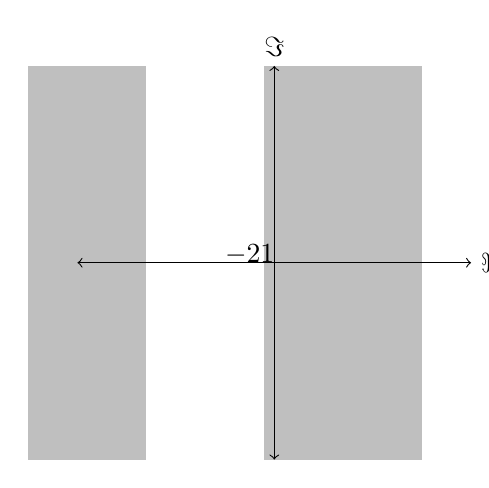
\begin{tikzpicture}
  \path [draw=none,fill=lightgray] (-2.5,-2.5)--(-1,-2.5)--(-1,2.5)--(-2.5,2.5)--cycle;
  \path [draw=none,fill=lightgray] (2.5,2.5)--(0.5,2.5)--(0.5,-2.5)--(2.5,-2.5)--cycle;
  \vtick{-1} node[pos=0.5,below] {$-2$};
  \vtick{0.5} node[pos=0.5,below] {$1$};
  \draw [<->] (-2.5,0) -- (2.5,0) node [right]  {$\Re$};
  \draw [<->] (0,-2.5) -- (0,2.5) node [above] {$\Im$};
\end{tikzpicture}
\end{center}
\end{solution}

\item \label{excer:laplacetransformcommonpolyut} Find the Laplace transform of the signal $t^n u(t)$ where $n\geq 0$ is an integer.
\begin{solution}
We have
\[
\calL\big(t^nu(t)\big) = \int_{-\infty}^{\infty} t^nu(t) e^{-st} dt = \int_{0}^{\infty} t^n e^{-st} dt.
\]
Integration by parts gives the indefinite integral
\[
\int t^n e^{-st} dt = \frac{t^n}{s} e^{-st} + \frac{n}{s} \int t^{n-1} e^{-st} dt.
\]
So, when $\Re(s) > 0$,
\begin{align*}
\calL\big(t^nu(t)\big) &= \lim_{t \to 0}\frac{t^n}{s} e^{-st} - \lim_{t \to \infty}\frac{t^n}{s} e^{-st} + \frac{n}{s} \int_{0}^\infty t^{n-1} e^{-st} dt \\
&= \frac{n}{s} \calL\big(t^{n-1}u(t)\big),
\end{align*}
since both limits converge to zero.  Unravelling the above recursive equation gives
\[
\calL\big(t^nu(t)\big) = \frac{n}{s}\times\frac{n-1}{s}\times\cdots\times\frac{1}{s}\times\calL\big(u(t)\big) = \frac{n!}{s^{n+1}}, \qquad \Re(s) > 0,
\]
since $\calL\big(u(t)\big) = \tfrac{1}{s}$ when $\Re(s) >0$. 
\end{solution}

\item Let $n \geq 0$ be an integer.  Show that the Laplace transform of the signal $(-t)^n u(-t)$ is the same as the Laplace transform of the signal $t^n u(t)$, but with a different region of convergence.
\begin{solution}
We have
\begin{align*}
\calL\big((-t)^nu(-t)\big) &= \int_{-\infty}^{\infty} (-t)^n u(-t) e^{-st} dt \\
&= \int_{-\infty}^{\infty} t^{n} u(t) e^{st} dt \qquad \text{(change variable t = -t)} \\
&= \calL( t^n u(t), -s) \qquad \Re(s) < 0 \\
&= \frac{n!}{s^{n+1}} \qquad \Re(s) < 0.
\end{align*}
\end{solution}

\item \label{exer:laplacetranstimeshift} Show that equation~\zeqref{eq:transferLaplcetheorem} on page~\zpageref{eq:transferLaplcetheorem} holds when the system $H$ the time shifter $T_\tau$. 
\begin{solution}
Put $y = T_\tau x = x(t- \tau)$.  Taking Laplace transforms
\begin{align*}
\calL y &= \calL T_\tau x \\
&= \int_{-\infty}^{\infty} T_\tau x(t) e^{-st} dt \\
&= \int_{-\infty}^{\infty} x(t - \tau) e^{-st} dt \\
&= \int_{-\infty}^{\infty} x(\kappa) e^{-s(\kappa + \tau)} d\kappa \qquad \text{(ch. vars. $\kappa = t - \tau$)} \\
&= e^{-s\tau}\int_{-\infty}^{\infty} x(\kappa) e^{-s\kappa} d\kappa \\
&= e^{-s\tau} \calL x \qquad s \in \roc(x) \\
&= \lambda T_\tau  \calL x \qquad s \in \roc(x)
\end{align*}
as required.  Observe that the region of convergence of $\calL y$ is the same as that of $\calL x$.
\end{solution}

\item \label{exer:laplacetransdiffproperty} Show that equation~\zeqref{eq:transferLaplcetheorem} on page~\zpageref{eq:transferLaplcetheorem} holds when the system $H$ is the differentiator under the added assumption that 
\[
\lim_{t\to\infty} x(t) e^{-st} = \lim_{t\to-\infty} x(t) e^{-st} = 0 \qquad \text{when $s \in \roc(x)$}.
\] 
\begin{solution}
% We now show the result for the differentiator $D$.  The argument we use is based on that of \citet[page~179]{Rudin_real_and_complex_analysis}.  We have just shown that the Laplace transform of the time shifted $T_{-\tau}(x,t) = x(t + \tau)$ is $e^{\tau s}\calL(x,s)$ with region of convergence $R_x$.  Since the Laplace transform is linear
% \[
% \calL\left( \frac{T_{-\tau}(x) - x}{\tau} \right) =  \frac{e^{\tau s} - 1}{\tau}\calL(x).
% \]
% We now consider what happens to both sides of this equation as $\tau \to 0$.  Application of L'Hopitals rule shows that
% \[
% \lim_{\tau \to 0}\frac{e^{\tau s} - 1}{\tau} = s,
% \]
% and so, the right hand side satisfies
% \[
% \lim_{\tau \to 0} \frac{e^{\tau s} - 1}{\tau}\calL(x) = s \calL(x).
% \]
% On the left hand side we have
% \[
% \lim_{\tau \to 0} \calL\left( \frac{T_{-\tau}(x) - x}{\tau} \right) = \lim_{\tau \to 0} \int_{-\infty}^\infty  \frac{x(t+\tau) - x(t)}{\tau} e^{-st} dt.
% \]
% Observe that
% \[
% \lim_{\tau \to 0} \frac{x(t+\tau) - x(t)}{\tau} = Dx
% \]
% by definition of the differentiator $D$.  Lebesgue's dominated convergence theorem~\cite[page~26]{Rudin_real_and_complex_analysis} can be used to justify exchanging limits and integration so that
% \begin{align*}
%  \lim_{\tau \to 0} \int_{-\infty}^\infty  \frac{x(t+\tau) - x(t)}{\tau} e^{-st} dt &=  \int_{-\infty}^\infty  \lim_{\tau \to 0} \frac{x(t+\tau) - x(t)}{\tau} e^{-st} dt \\
% &= \int_{-\infty}^\infty D x(t) e^{-st} dt = \calL D x.
% \end{align*}
% We now have  $\calLDx = s\calLx = \lambda D \calL x$ as required.

Put $y = Dx$.  Taking Laplace transforms
\[
\calL y = \calL D x = \int_{-\infty}^{\infty} Dx(t) e^{-st} dt.
\]
Integrating by parts 
\[
\calL y = \big[ x(t) e^{-st} \big]_{-\infty}^\infty + s\int_{-\infty}^{\infty} x(t) e^{-st} dt = \big[ x(t) e^{-st} \big]_{-\infty}^\infty + s\calL x.
\]
and, by assumption, 
\[
\big[ x(t) e^{-st} \big]_{-\infty}^\infty = \lim_{t\to\infty} x(t) e^{-st}  - \lim_{t\to-\infty} x(t) e^{-st} = 0
\] 
whenever $s$ is in the region of convergence of $x$.  In this case $\calL y = s\calL x$ as required.

The result follows for the $k$th differentiator $D^k$ under the assumption that
\[
\lim_{t\to\infty} D^{c}x(t) e^{-st} = 0 \qquad \text{and} \qquad \lim_{t\to-\infty} D^{c}x(t) e^{-st} = 0
\]
for all $c = 1, 2, \dots, k-1$ because
\[
\calL D^k x = \calL D D^{k-1} x= s \calL D^{k-1}x 
\]
and unravelling this recursion gives
\[
\calL D^k y  = \underbrace{s \times s \times \dots \times s}_{\text{$k-1$ times}} \times \calL D y = s^k \calL y  = \lambda D^k \calL y.
\]
\end{solution}


\item What is the transfer function of the integrator system $I_\infty$?  What is the domain of this transfer function? 
\begin{solution}
We can do this in two ways.  First by obtaining the transfer function directly and second by using the fact that the impulse response of $I_\infty$ is the step signal $u$ (Section~\zref{sec:conv-regul-syst}).

Recall from Section~\zref{sec:some-import-syst} that by default the domain of $I_\infty$ is the set of locally integrable signals $x$ for which the integral $\int_{-\infty}^0 \abs{x(t)} dt$.  This set of precisley $\dom u$ (see also Exercise~\ref{exer:domuislcoalinintneg}).  Observe first that $e^{st} \in \dom u$ if and only if the real part of $s$ is nonegative.  Thus, the domain of the transfer function $\lambda I_{\infty}$ is the set of complex numbers $s$ with $\Re s > 0$.  The response of $I_\infty$ to $e^{st}$ is
\[
I_\infty(e^{st}) = \int_{-\infty}^t e^{s\tau} d\tau = \frac{e^{st}}{s} - \lim_{t\to -\infty}\frac{e^{st}}{s}
\]
and the limit exists only when $\Re{s} > 0$ and in this case it is zero.  So
\[
I_\infty(e^{st}) = \frac{1}{s} e^{st} \qquad \Re{s} > 0
\]
and $\lambda I_\infty(s) = \tfrac{1}{s}$.

The second approach is to use that $\lambda H = \calL u$.  We have, from Section~\ref{sec:regions-convergence}, that that the Laplace transform of the signal $e^{\alpha t} u(t)$ takes the form
\[
\calL(e^{ \alpha t}u(t)) = \frac{1}{s-\alpha} \qquad \Re s > \Re \alpha.
\]
Setting $\alpha = 0$ we find that
\[
\calL u(s) = \lambda I_\infty(s) = \frac{1}{s} \qquad \Re s > 0
\]
as before.
\end{solution}


\item \label{exer:partialfracfirstorder} By partial fractions, or otherwise, assert that
\[
\frac{as}{s+b} = a - \frac{ab}{s+b}
\]
\begin{solution}
Adding and subtracting $ab$ from the numerator
\[
\frac{as+ab-ab}{s+b} = \frac{a(s+b)-ab}{s+b} = \frac{a(s+b)}{s+b} - \frac{ab}{s+b} = a - \frac{ab}{s+b}
\]
\end{solution}

\item \label{exer:partialfracsecondorder} By partial fractions, or otherwise, assert that
\[
\frac{s + c}{(s+a)(s+b)} = \frac{a-c}{(a-b)(s+a)} + \frac{c-b}{(a-b)(s+b)}
\]
\begin{solution}
Hypothesise the solution
\[
\frac{s + c}{(s+a)(s+b)} = \frac{A}{s+a} + \frac{B}{s+b}.
\]
Multiplying both sides by $(s+a)(s+b)$,
\[
s+c = A(s+b) + B(s+a).
\]
Putting $s = -a$ gives $c-a = A(b-a)$, and pitting $s=-b$ gives $c-b = B(a-b)$, and so,
\[
\frac{s+c}{(s+a)(s+b)} = \frac{a-c}{(a-b)(s+a)} + \frac{c-b}{(a-b)(s+b)}.
\]
\end{solution}

\begin{hardexercise}

\item \label{exer:partialfracfourthorder} By partial fractions, or otherwise, assert that
\[
\frac{1}{s(s-a)(s-b)(s-b^*)} = \frac{A_0}{s} + \frac{A_1}{s-a} + \frac{A_2}{s-b} + \frac{A_2^*}{s-b^*}
\]
where $a \in \reals$ and $b \in \complex$ and $\Im(b) \neq 0$ and
\[
A_0 = -\frac{1}{a\sabs{b}^2}, \qquad A_1 =  \frac{1}{a\sabs{a - b}^2}, \qquad A_2 = \frac{1}{b(b-a)(b-b^*)}.
\]
You might wish to check your solution using a symbolic programming language (for example Sage, Mathematica, or Maple).
\begin{solution}
The mathemtica command
\begin{verbatim}
Apart[1/s/(s - a)/(s - b)/(s - c), s]
\end{verbatim}
or the maxima command
\begin{verbatim}
partfrac(1/s/(s - a)/(s - b)/(s - c), s)
\end{verbatim}
returns the equation
\[
\frac{1}{s(s-a)(s-b)(s-c)} = \frac{A_0}{s} + \frac{A_1}{s-a} + \frac{A_2}{s-b} + \frac{A_3}{s-c}
\]
where
\[
A_0 = -\frac{1}{abc}, \qquad A_1 =  \frac{1}{a (a-b) (a-c)}, 
\]
\[
A_2 = \frac{1}{b (b-a) (b-c)}, \qquad A_3 = \frac{1}{c (c-a) (c-b)}.
\]
Setting $c = b^*$ gives
\[
A_0 = -\frac{1}{a\sabs{b}^2}, \qquad A_1 =  \frac{1}{a\sabs{a - b}^2}, 
\]
\[ 
A_2 = \frac{1}{b(b-a)(b-b^*)}, \qquad A_3 = \frac{1}{b^*(b^*-a)(b^*-b)} = A_2^*
\]
as required.
\end{solution}

\end{hardexercise}

\item Let $y$ be a signal with Laplace transform taking the form
\[
\calL y(s) = \frac{2s + 1}{s^2 + s - 2}
\]
By partial fractions, or otherwise, find all possible signals $y$ with this Laplace transform and the corresponding region of convergence. 
\begin{solution}
Factorise the polynomial on the denominator
\[
\frac{2s + 1}{(s+2)(s-1)}.
\]
Adding and subtracting $s-1$ on the numerator 
\begin{align*}
\frac{2s + 1 + (s-1) - (s-1)}{(s+2)(s-1)} &= \frac{s-1}{(s-1)(s+2)} + \frac{s+2}{(s-1)(s+2)} \\
&= \frac{1}{s+2} + \frac{1}{s-1}.
\end{align*}
There are two time domain signals with Laplace transform $\frac{1}{s+2}$,
\[
e^{-2t} u(t), \; \Re(s) > -2 \qquad \text{and} \qquad -e^{-2t}u(-t), \; \Re(s) < -2,
\] 
and two time domain signals with Laplace transform $-\frac{1}{s-1}$,
 \[
e^{t}u(t), \; \Re(s) > 1 \qquad \text{and} \qquad -e^{t} u(-t), \; \Re(s) < 1.
\] 
There are three possible signals with nonempty regions of convergence
\[
y(t) = e^{-2t} u(t) - e^{t} u(-t) \qquad -2 < \Re(s) < 1,
\]
\[
y(t) = e^{-2t} u(t) + e^{t} u(t) \qquad 1 < \Re(s),
\]
\[
y(t) = - e^{-2t} u(-t) - e^{t} u(-t) \qquad \Re(s) < -2.
\]
\end{solution}

\item \label{excer:timescalelaplace} Let $x$ be a signal.  Show that the time scaled signal $x(\alpha t)$ with $\alpha \neq 0$ satisfies equation~\zeqref{eq:timescalingpropertrylaplacetrans} on page~\zpageref{eq:timescalingpropertrylaplacetrans}.
\begin{solution}
First consider when $\alpha = -1$ so that $x(-t)$ is the reflection of the signal $x$ in time (see Section~\zref{sec:some-import-syst}).  We have 
\begin{align*}
 \calL\big( x(-t), s \big) &=  \int_{-\infty}^{\infty} x(-t)  e^{-s t} dt \\
 &=  -\int_{\infty}^{-\infty} x(\tau)  e^{s\tau} d\tau & \text{(change variable $\tau = -t$)}\\
 &=  \int_{-\infty}^{\infty} x(\tau)  e^{ s \tau} d\tau = \calL(x, -s) \qquad \Re(-s) \in R.
 \end{align*}
 This special case is called the \term{time reversal property}.  Now, when $\alpha > 0$,
 \begin{align*}
 \calL\big( x(\alpha t), s \big) &=  \int_{-\infty}^{\infty} x(\alpha t)  e^{-s t} dt \\
 &=  \frac{1}{\alpha} \int_{\infty}^{\infty} x(\tau)  e^{-s \tau / \alpha}  d\tau & \text{(change variable $\tau = \alpha t$)}\\
 &= \frac{1}{\alpha} \calL(x, s / \alpha) \qquad \Re(s/\alpha) \in R.
 \end{align*}
Combining this with the time reversal property we obtain
 \[
 \calL\big(x(\alpha t),s\big) = \frac{1}{\abs{\alpha}} \calL(x, s/\alpha), \qquad a \neq 0, \Re(s/\alpha) \in R.
 \]
as required.
\end{solution}

% \item \label{exer:numericalintactiverc} Show that the following integrals are equal
% \[
% r \int_{0}^\infty e^{-r\tau} \sinc( t - F\tau ) d\tau = \frac{1}{2\pi}\int_{-\pi}^{\pi} \frac{\cos(\omega F t) + \omega t \sin(\omega F t)}{1 - V^2\omega^2t^2} \; dt
% \]
% where $V = \tfrac{F}{r}$ and $r > 0$.  (Hint: use that $\sinc(t) = \int_{-1/2}^{1/2} e^{-j2\pi ft} df$ from~\eqref{eq:sincandrect} on page~\pageref{eq:sincandrect}).
% \begin{solution}
% It is helpful to first make the change of variable $k = r \tau$ so that the integral on the left hand side is
% \[
% \int_{0}^\infty e^{-k} \sinc( t - Vk ) dk
% \]
% because $r > 0$.  Using the hint we can write this as a double integral
% \begin{align*}
% \int_{0}^\infty e^{-\tau} \sinc( t - Vk ) dk &= \int_{0}^\infty e^{-k} \int_{-1/2}^{1/2} e^{-j2\pi f (t-Vk)} \; df \; dk \\
%  &= \int_{0}^\infty \int_{-1/2}^{1/2} e^{-j2\pi f (t-Vk) - k} \; df \; dk.
% \end{align*}
% Exchanging the order of integration we obtain
% \begin{align*} 
%  \int_{-1/2}^{1/2} \int_{0}^\infty e^{-j2\pi f (t-Vk) -k} \; dk \; df = \int_{-1/2}^{1/2} e^{-j2\pi f t} \int_{0}^\infty e^{(j 2\pi V f - 1)\tau} \; dk \; df \\
% \end{align*}
% The inner integral satisfies
% \[
%  \int_{0}^\infty e^{(j 2\pi f V - 1)k} \; dk = \left. \frac{e^{(j 2\pi f V - 1)k}}{j 2\pi f V - 1} \right\vert_0^\infty = -\frac{1}{j 2\pi f V - 1}.
% \]
% from which we obtain
% \[
% -\int_{-1/2}^{1/2} \frac{e^{-j2\pi f t}}{j 2\pi f V - 1} \; df
% \]
% Letting $\omega = 2\pi f$ and changing variable we have
% \[
% r \int_{0}^\infty e^{-r\tau} \sinc( t - F\tau ) d\tau = \frac{1}{2\pi} \int_{-\pi}^\pi \frac{e^{-j \omega t}}{1 - j V \omega} \; d\omega.
% \]
% The integral is real valued and so we may take the real part inside the integral on the right hand side.  Using the fact that $\Re(x) = x + x^*$ for $x 
% \in \complex$ we have
% \begin{align*}
% \Re\left(\frac{e^{-j \omega t}}{1 - j V \omega}\right) &= \frac{e^{-j \omega t}}{1 - j V \omega} + \frac{e^{j \omega t}}{1 + j V \omega} \\
% &= \frac{e^{-j \omega t}(1 + j V \omega) + e^{j \omega t}(1 - j V \omega)}{(1 - j V \omega)(1 + j V \omega)} \\
% &= \frac{e^{-j \omega t} + e^{j \omega t} - j V \omega(e^{j \omega t} - e^{-j \omega t})}{1 + V^2 \omega^2} \\
% &= 2 \frac{\cos(\omega t) + V \omega \sin(\omega t)}{1 + V^2 \omega^2}.
% \end{align*}
% This leads to
% \[
% r \int_{0}^\infty e^{-r\tau} \sinc( t - F\tau ) d\tau = \frac{1}{\pi} \int_{-\pi}^\pi \frac{\cos(\omega t) + V \omega \sin(\omega t)}{1 + V^2 \omega^2} \; d\omega.
% \]
% \end{solution}

% \item \label{exer:thetainfinitelydiff} Plot the signal $\theta(t)$ from~\eqref{eq:thetainfinitediff} and its first 2 derivatives $D \theta$ and $D^2 \theta$. Show that this signal is infinitely differentiable, that is, that it can be differentiated as many times as you like.
% \begin{solution}

% \end{solution}

% \item \label{exer:elevatorgeneralequation} Show that the response of the DC motor to input voltage $v$ from~\eqref{eq:velevatordesigned} satisfies~\eqref{eq:generalequationelevator}.  That is, show that convolution of the impulse response of the motor $h(t) = \tfrac{1}{a} u(t)\big( 1 - e^{-a t/b}\big)$ and the voltage signal $v$ is given by~\eqref{eq:generalequationelevator}.  You may wish to use a symbol programming language (for example Sage, Mathematica, or Maple).
% \begin{solution}
% The following Mathematica commands immediately yield this solution
% \begin{verbatim}
% Theta[t_] := (UnitStep[t] - UnitStep[t - Pi])*Pi*(1-Cos[t]) + 2*Pi*UnitStep[t - Pi];
% v[t_] := 2*Theta'[t] + 3*Theta''[t];
% h[t_, a_, b_] := UnitStep[t]*(1 - Exp[-a/b*t])/a;
% FullSimplify[
% Integrate[
%   h[Tau, a, b]*v[t - Tau], {Tau,-Infinity,Infinity}, 
%   Assumptions -> t Element Reals]]
% \end{verbatim}
% \end{solution}

\item Consider the active electrical circuit from Figure~\zref{elec:activeRC} described by the differential equation from~\zeqref{eq:twoaparrarrelRCactive}.  Derive the transfer function of this system.  Find an explicit system $H$ that maps the input voltage $x$ to the output voltage $y$.  State whether this system is stable and/or regular.
\begin{solution}
The differential equation modelling the circuit is
\[
-\frac{x}{R_1} - C_1 D x = \frac{y}{R_2} + C_2 D y,
\]
and taking Laplace transforms on both sides of this equation
\[
\calL{y} = -\frac{\tfrac{1}{R_1} + C_1s}{\tfrac{1}{R_2} + C_2s} \calL(x) = -\frac{\alpha + \gamma s}{\beta + s}
\]
where $\alpha = \tfrac{1}{R_1C_2}$, $\beta = \tfrac{1}{R_2C_2}$, and $\gamma = \tfrac{C_1}{C_2}$.  The transfer function of the system mapping $x$ to $y$ is correspondingly
\[
\lambda(H) = -\frac{\alpha + \gamma s}{\beta + s} = -\frac{\alpha}{\beta + s} - \frac{\gamma s}{\beta + s}
\]
Applying partial fraction (as in Exercise~\ref{exer:partialfracfirstorder}) to the second term gives
\[
\lambda(H) = -\frac{\alpha + \gamma\beta}{\beta + s} - \gamma
\]
The first term $-\frac{\alpha + \gamma\beta}{\beta + s}$ corresponds with a regular system, say $H_2$, having impulse response
\[
h_2 = -(\alpha + \gamma\beta) u(t) e^{-\beta t}
\]
by using the Laplace transform pair from~\zeqref{eq:laplacetneucommon} with the integer $n=0$.  The term $-\gamma$ correspond with the system $H_1 = \gamma T_0$, i.e, the identity system multiplied by $-\gamma$.  The system $H$ that describes the mapping between input voltage $x$ and output voltage $y$ is thus
\[
H(x) = H_1(x) + H_2(x) = -\gamma x + h_2 * x.
\]
The system is not regular because the $H_1$ is not regular.  The system is stable because $H_1$ is stable and $H_2$ is stable because the impulse response $h_2$ is absolutely integrable since $\beta = \tfrac{1}{R_2C_2} > 0$.  Equivalently the system is not regular because the transfer function does not have more poles than zero, and the system is stable because the transfer function has at least as many poles as zeros (equal in this case), and because all the poles lie strictly in the left half plane. 
\end{solution}

\begin{hardexercise}
\item \label{exer:massspringdamperrect} Given the mass spring damper system described by~\zeqref{eq:masspringeqseclapltrans}, find the position signal $p$ given that the force signal 
\[
f(t) = \rect\big(t-\tfrac{1}{2}\big) = \begin{cases}
1 & 0 < t \leq 1 \\
0 & \text{otherwise}
\end{cases}
\]
is the rectangular function time shifted by $\tfrac{1}{2}$.  Consider three cases:
\begin{enumerate}
\item $M=1$, $K=\tfrac{\pi^2}{4}$ and $B=\tfrac{\pi}{3}$,
\item $M=1$, $K=\tfrac{\pi^2}{4}$ and $B=\pi$,
\item $M=1$, $K=\tfrac{\pi^2}{4}$ and $B=2\pi$,
\end{enumerate}
Plot the solution in each case, and comment on whether the system is underdamped, overdamped, or critically damped. 
\begin{solution}
Observe that the input force signal can be written as the sum of the step function $u$ and its negated time-shift, that is,
\[
f(t) = u(t) - u(t - 1) = u(t) - T_{1} u(t)
\]
and so, the response of the linear, time invariant system $H$ modelling the mass spring damper to input force signal $f$ is
\[
Hf = H(u - T_{1}u) = Hu - T_{1}Hu,
\]
and so, $Hf(t) = Hu(t) - Hu(t-1)$, where $Hu$ is the step response of the system.  The step responses are described in Section~\zref{sec:second-order-systems}.  As described in Section~\zref{sec:second-order-systems}, the system is underdamped when $B = \tfrac{\pi}{3}$, critically damped when $B = \pi$ and overdamped when $B = 2\pi$.
\end{solution}
\end{hardexercise}

\item Plot the signal $x(t) = \sin(t e^t) u(t)$ and find and plot its derivative $D x$.  Show that the region of convergence of $x$ contains those complex numbers $s$ with $\Re s > 0$ and that the region of convergence of $D x$ contains those with $\Re s > 1$.
\begin{solution}
By application of the chain rule the derivative of $\sin(t e^t)$ is $(t+1)e^t \cos(e^t) u(t)$.  These signals are plotted below.
\begin{center}
\begin{tikzpicture}
\begin{scope}[xscale=1.5]
    \draw[->] (-0.5,0) -- (2.8,0) node[above] {$t$};
    \draw[->] (0,-1.3) -- (0,1.3) node[above right] {$\sin(t e^t) u(t)$};
    \draw[thick] (-0.25,0) -- (0,0);
    \draw[smooth,color=black,domain=0:2.5,thick,samples=300] plot function{sin(x*exp(x))};
\end{scope}
\htick{1} node[pos=0.5,left] {$1$};
\htick{-1} node[pos=0.5,left] {$-1$};
\end{tikzpicture}
\end{center}
\begin{center}
\begin{tikzpicture}
\begin{scope}[xscale=1.5,yscale=0.05]
    \draw[->] (-0.5,0) -- (2.8,0) node[above] {$t$};
    \draw[->] (0,-40.3) -- (0,40.3) node[above right] {$(t+1)e^t \cos(t e^t) u(t)$};
    \draw[thick] (-0.25,0) -- (0,0);
    \draw[smooth,color=black,domain=0:2.5,thick,samples=300] plot function{(1+x)*exp(x)*cos(x*exp(x))};
    \draw[smooth,color=black,domain=0:2.45,thick,samples=50,dashed] plot function{(1+x)*exp(x)};
    \draw[smooth,color=black,domain=0:2.45,thick,samples=50,dashed] plot function{-(1+x)*exp(x)};
\end{scope}
\begin{scope}[yscale=0.05]
\htick{30} node[pos=0.5,left] {$30$};
\htick{-30} node[pos=0.5,left] {$-30$};
\end{scope}
\end{tikzpicture}
\end{center}

We have $\abs{x(t)} = \abs{\sin(t e^t) u(t)} < 1$ for all $t \in \reals$ and so
\begin{align*}
\calL\big( x , s\big) &= \int_{-\infty}^\infty \sin(t e^t) u(t) e^{-s t} dt \\
&= \int_{0}^\infty \sin(t e^t) e^{-s t}  dt \\
&\leq = \int_{0}^\infty \abs{\sin(t e^t) e^{-s t}}  dt \\
&\leq \int_{0}^\infty e^{-\Re(s) t}  dt
\end{align*}
which is finite for all $s$ with $\Re(s) > 0$ as required.  For the derivative we have
\begin{align*}
\calL D x (s) &= \int_{-\infty}^\infty (t+1)e^t \cos(t e^t) u(t) e^{-s t} dt \\
&= \int_{0}^\infty (t+1) \cos(t e^t) e^{-(s-1) t}  dt \\
&\leq \int_{0}^\infty \abs{(t+1) \cos(t e^t) e^{-(s-1) t}}  dt \\
&\leq \int_{0}^\infty (t+1) e^{-(\Re(s)-1) t}  dt
\end{align*}
which is finite for all $s$ with $\Re(s) > 1$ as required.
\end{solution}

\item \label{exer:eReslimsinclike} Show that the limit as $\abs{s} \to 0$ of 
\[
\frac{ e^{s/2} - e^{-s/2}}{s}
\]
is equal to $1$.

\begin{hardexercise}
\item \label{exer:twomassspringtwowallstranfuncpolezeros} Consider the mechanical system in Figure~\ref{mech:twomassspringtwowalls} from Exercise~\ref{exer:twomassspringtwowalls}.  After solving Exercise~\ref{exer:twomassspringtwowalls}, find the transfer function of a linear shift-invariant $H$ system mapping $f$ to $p$.  Now suppose that $M_1 = K_1 = K_2 = B = 1$ and $M_2 = 2$.  Find the poles and zeros of $H$ and draw a pole zero plot.  Determine whether $H$ is stable and/or regular.  Find and plot the impulse response and the step response of $H$ if they exist.

\begin{solution}
Let $H$ be a linear time invariant system mapping $f$ to $p$.  The transfer function of $H$ is
\[
\lambda H(s) = \frac{1}{1 + 2s + 4s^2 + 2s^3 + 2s^4}.
\]
Factorising the polynomial on the denominator we obtain
\[
\lambda H(s) = \frac{1}{(s-\beta_0)(s-\beta_1)(s-\beta_2)(s-\beta_3)}
\]
where the roots are
\[
\beta_0 = \beta_1^* = -0.193622 + 1.17046j, \;\;\; \beta_2 = \beta_3^* = -0.306378 + 0.511255j
\]
The system has no zeros and four poles.  A pole zero plot is shown below.  

\begin{center}
  \begin{tikzpicture}
\begin{scope}[yscale=1.5,xscale=10]
    % \path [draw=none,fill=lightgray] (-2.5,-2.5)--(-1,-2.5)--(-1,2.5)--(-2.5,2.5)--cycle;
    %\vtick{-1} node[pos=0.5,below] {$-2$};
    \poletikz{-0.193622}{1.17046} \node[above left] at (-0.193622,1.17046) {$\beta_0$};
    \poletikz{-0.193622}{-1.17046} \node[above left] at (-0.193622,-1.17046) {$\beta_1$};
    \poletikz{-0.306378}{0.511255} \node[above left] at (-0.306378,0.511255) {$\beta_2$};
    \poletikz{-0.306378}{-0.511255} \node[above left] at (-0.306378,-0.511255) {$\beta_3$};
    %\poletikz{-5/11}{0} \node[above left] at (-5/11,0) {$-\tfrac{5}{11}\times 10^4$};
    \polezeroaxis{0.5}{2};
\end{scope}
\begin{scope}[yscale=1.5]
\htick{1} node[pos=0.5,right] {$1$};
\htick{-1} node[pos=0.5,right] {$-1$};
\end{scope}
\begin{scope}[xscale=10]
\vtick{-0.1} node[pos=0.5,below] {$-\tfrac{1}{10}$};
\vtick{-0.2} node[pos=0.5,below] {$-\tfrac{2}{10}$};
\vtick{-0.3} node[pos=0.5,below] {$-\tfrac{3}{10}$};
%\vtick{-0.4} node[pos=0.5,below] {$-\tfrac{4}{10}$};
\end{scope}
  \end{tikzpicture}
\end{center}

Because there are atleast as many poles as zeros and the real part of all the poles is negative the system is stable.  Because there are more poles than zeros the system is regular and has an impulse response.  Applying partial fractions gives
\[
\lambda H(s) = \frac{A_0}{s - \beta_0} + \frac{A_1}{s - \beta_1} + \frac{A_2}{s - \beta_2} + \frac{A_3}{s - \beta_3}
\]
where
\[
A_0 = A_1^* = -0.0887401 + 0.368434 j, \;\;\; A_2 = A_3^* = 0.0887401 + 0.863059j.
\]
The impulse response is
\[
h(t) = u(t) \left( A_0 e^{\beta_0 t} + A_1 e^{\beta_1 t} + A_2 e^{\beta_2 t} + A_3 e^{\beta_3 t}  \right).
\]
The step response is
\[
H u = I_\infty h = u(t) \left( C_0 e^{ \beta_0 t} + C_1 e^{\beta_1 t} + C_2 e^{\beta_2 t} + C_3 e^{\beta_3 t} - B  \right)
\]
where $C_n = A_n/\beta_n$, $n = 0,1,2,3$ and $B=C_0+C_1+C_2+C_3$.  These responses are plotted below.

\begin{center} 
  {
    \def\Azeroabs{0.37897}
    \def\Azeroarg{-1.80715}
    \def\Atwoabs{0.867609}
    \def\Atwoarg{-1.46834}
    \def\betazerore{-0.193622}
    \def\betazeroim{-1.17046}
    \def\betatwore{-0.306378}
    \def\betatwoim{0.511255}
    \def\Czeroabs{0.319438}
    \def\Czeroarg{-0.0724163}
    \def\Ctwoabs{1.45565}
    \def\Ctwoarg{2.70417}
    \def\B{-2}
    \def\step(#1){ifthenelse(#1>0,1,0)}
    \def\h(#1){2*\step(#1)*(\Azeroabs*exp(\betazerore*#1)*cos(180/3.145*(\betazeroim*#1 + \Azeroarg)) + \Atwoabs*exp(\betatwore*#1)*cos(180/3.145*(\betatwoim*#1 + \Atwoarg)))}
    \def\Hu(#1){\step(#1)*(2*\Czeroabs*exp(\betazerore*#1)*cos(180/3.145*(\betazeroim*#1 + \Czeroarg)) + 2*\Ctwoabs*exp(\betatwore*#1)*cos(180/3.145*(\betatwoim*#1 + \Ctwoarg)) - \B)}

    \begin{tikzpicture}
      \begin{scope}[xscale=0.5,yscale=2]
        \draw[->] (-2,0) -- (17,0) node[above] {$t$};
        \draw[->] (0,-0.7) -- (0,1.3) node[right] {$h$};
        \draw[thick] (-1,0) -- (0,0);
        \draw[color=black,thick] plot[domain=0:15.5,samples=101] (\x,{\h(\x)});
      \end{scope}
      \begin{scope}[xscale=0.5]
        \vtick{5} node[pos=0.5,below] {$5$};
        \vtick{10} node[pos=0.5,below] {$10$};
        \vtick{15} node[pos=0.5,below] {$15$};
      \end{scope}
      \begin{scope}[yscale=2]
        \htick{1} node[pos=0.5,left] {$1$};
      \end{scope}
    \end{tikzpicture}

    \vspace{0.5cm}

    \begin{tikzpicture}
      \begin{scope}[xscale=0.5,yscale=1]
        \draw[->] (-2,0) -- (17,0) node[above] {$t$};
        \draw[->] (0,-0.3) -- (0,3.1) node[right] {$H(u)$};
        \draw[thick] (-1,0) -- (0,0);
        \draw[color=black,thick] plot[domain=0:15.5,samples=101] (\x,{\Hu(\x)});
      \end{scope}
      \begin{scope}[xscale=0.5]
        \vtick{5} node[pos=0.5,below] {$5$};
        \vtick{10} node[pos=0.5,below] {$10$};
        \vtick{15} node[pos=0.5,below] {$15$};
      \end{scope}
      \htick{1} node[pos=0.5,left] {$1$};
      \htick{2} node[pos=0.5,left] {$2$};
    \end{tikzpicture}
  }
\end{center}

\end{solution}
\end{hardexercise}

\item \label{exer:dcmotorpotfeedbacktranfunc} Consider the electromechanical system in Figure~\ref{fig:dcmotorpotfeedback} from Exercise~\ref{exer:dcmotorpotfeedback}.  After solving Exercise~\ref{exer:dcmotorpotfeedback}, find the transfer function of a linear shift-invariant system that maps the input voltage $v$ to the motor angle $\theta$.  Under the assumption that the motor coefficients satisfy $L=0$ and $K_b=K_\tau=B=R=J=1$ draw a pole zero plot and determine whether this system is stable and/or regular.  Find and plot the impulse response and step response if they exist.

\begin{solution}
Exercise~\zref{exer:dcmotorpotfeedback} finds the following differential equation relating $v$ and $\theta$,
\[
v = \theta + \left(\frac{RB}{K_\tau} + K_b\right) D \theta + \frac{RJ}{K_\tau} D^2 \theta.
\]
The transfer function is
\[
\frac{1}{1 + \left(\frac{RB}{K_\tau} + K_b\right) s  + \frac{RJ}{K_\tau} s^2}.
\]
Under the assumption that $K_b=K_\tau=B=R=J=1$ the transfer function is
\[
\frac{1}{1 + 2s  + s^2} = \frac{1}{(1 + s)^2}.
\]
There are two equal real poles at $s = -1$ and no zeros.  A pole zero plot is below.

\begin{center}
  \begin{tikzpicture}
    \poletikz{-1}{0} \node[below] at (-1,0) {$-1$};
    \polezeroaxis{2}
  \end{tikzpicture}
\end{center}

The system is regular because there are more poles than zeros.  The system is stable because there are at least as many poles as zeros and all poles have negative real part.  The impulse response is found to be $h(t) u(t) t e^{-t}$ by application of the inverse Laplace transform.  The step response is given by application of the integrator system
\[ 
Hu = I_\infty(h) = \int_{-\infty}^t u(\tau) t e^{-\tau} d\tau = \int_{0}^t t e^{-\tau} d\tau = u(t) \big( 1 - e^{-t}(t+1) \big).
\] 
These responses are plotted below

\begin{center}
\begin{tikzpicture}
\begin{scope}[yscale=4]
    \draw[->] (-1,0) -- (10,0) node[above] {$t$};
    \draw[->] (0,-0.1) -- (0,0.5) node[right] {$u(t) t e^{-t}$};
    \draw[thick] (-0.5,0) -- (0,0) {};
    \draw[color=black,thick] plot[domain=0:9,samples=101,smooth] function{x*exp(-x)};
    \htick{0.3} node[pos=0.5,left] {$0.3$};
\end{scope}
    \vtick{1} node[pos=0.5,below] {$1$};
    \vtick{7} node[pos=0.5,below] {$7$};
\end{tikzpicture}

\begin{tikzpicture}
\begin{scope}[yscale=2]
    \draw[->] (-1,0) -- (10,0) node[above] {$t$};
    \draw[->] (0,-0.2) -- (0,1.3) node[right] {$u(t) \big( 1 - e^{-t}(t+1) \big)$};
    \draw[thick] (-0.5,0) -- (0,0) {};
    \draw[color=black,thick] plot[domain=0:9,samples=101,smooth] function{1-(x+1)*exp(-x)};
    \htick{1} node[pos=0.5,left] {$1$};
\end{scope}
    \vtick{1} node[pos=0.5,below] {$1$};
    \vtick{7} node[pos=0.5,below] {$7$};
\end{tikzpicture}
\end{center}

\end{solution}

\begin{reallyhardexercise}
\item \label{exer:finhandroch} Let $x$ be a signal.  Show that the complex exponential signal $e^{st} \in \dom x$ if and only if the signal $x(t)e^{-st}$ is absolutely integrable.
\begin{solution}
The set $\dom x$ contains all those signals such that
\[
\int_{-\infty}^{\infty} \abs{x(\tau) x(t - \tau} d\tau < \infty  \qquad \text{for all $t \in \reals$}.
\]
If $e^{st} \in \dom x$ then
\[
\int_{-\infty}^{\infty} \abs{x(\tau) e^{s(t - \tau)}} d\tau = \abs{e^{st}} \int_{-\infty}^{\infty} \abs{x(\tau) e^{-s \tau}} d\tau < \infty  \qquad \text{for all $t \in \reals$}.
\]
Setting $t = 0$ we find that
\[
\int_{-\infty}^{\infty} \abs{x(\tau) e^{-s \tau}} d\tau < \infty
\] 
and so $x(t) e^{-st}$ is absolutely integrable.  On the other hand, if $x(t) e^{-st}$ is absolutely integrable then
\[
\int_{-\infty}^{\infty} \abs{x(\tau) e^{s(t - \tau)}} d\tau = \abs{e^{st}} \| x(t) e^{-st}\|_1 < \infty  \qquad \text{for all $t \in \reals$}.
\]
since $e^{st}$ is finite for all $t$, and so, $e^{st} \in \dom x$.
\end{solution}


\item \label{exer:domfgrocfrocg} Show that the complex exponential signal $e^{st} \in \dom f\;g$ if and only if $s \in \roc f \cap \roc g$, that is, $\cep \dom f\;g = \roc f \cap \roc g$.

\end{reallyhardexercise}

\end{excersizelist}

%%% Local Variables: 
%%% mode: latex
%%% TeX-master: "main.tex"
%%% End: 